\section{Basic Block Collection and Classification}
\subsection{Basic Block Collection}
We selected the source applications of our basic blocks with two goals:
\begin{enumerate*}
    \item The set of applications should cover a diverse range
of domains to represent real world workload
    \item Their basic blocks should reflect input that concerns typical users of a performance model;
    compiler developers deals with
    basic blocks from general purpose programs,
    which have different characteristics
    than those from 
    high performance kernels. 
\end{enumerate*}
Table~\ref{tab:apps} shows the applications from which we extracted basic blocks.

\begin{table}
\begin{tabular}{|p{0.4\columnwidth}|p{0.4\columnwidth}|}
\hline
Application & Domain \\

\hline
OpenBlas & Scientific Computing \\

\hline
Redis & Database \\

\hline
SQLite & Database \\

\hline
GZip & Compression \\

\hline
TensorFlow & Machine Learning \\

\hline 
Clang/LLVM & Compiler \\

\hline
Eigen & Scientific Computing \\

\hline
Embree & Ray Tracing\\

\hline
FFmpeg & Multimedia\\
\hline
\end{tabular}
\\
\caption{Source applications of basic blocks}
\label{tab:apps}
\end{table}

We selected Clang/LLVM\cite{llvm} (compiler),
Redis (in-memory database), SQLite (database), and Gzip (compression)
to collect basic blocks that represent
applications that are written in general purpose languages
like C and C++.
Basic blocks from these programs
typically have high memory traffic, and are usually not-vectorized.
We chose these applications because they are some of the mostly used
applications today; they are well tuned for performance;
and they all have sophisticated use of algorithms and data structures,
giving us a large source of diverse basic blocks.

We selected high performance kernels from the following domains:
cryptography (OpenSSL), scientific computing (OpenBLAS and Eigen),
machine learning (TensorFlow\cite{tensorflow}),
and rendering/multimedia (Embree\cite{embree} and FFmpeg).
OpenSSL, OpenBLAS, and FFmpeg use handwritten assembly for performance critical inner loops.
Embree is written in ispc\cite{ispc}, a data parallel language
designed specifically to target Intel's vector extensions.

We collected basic blocks from these applications using
a dynamic analysis implemented in DynamoRIO\cite{dynamorio},
which provides an API to record every basic block
executed at runtime.
We opted for dynamic analysis rather than static disassembly
because precise static disassembly of x86 binary
is undecidable.
We use the official benchmark suites of these applications\footnote{
Except for FFmpeg and Gzip, which to the best of our knowledge do not have
official benchmarks. For these two applications we use inputs
from https://openbenchmarking.org.
} to simulate realistic execution of these applications when performing
the dynamic analysis.
We evaluated Eigen on two sparse linear algebra workloads:
sparse matrix-matrix multiplication (SPMM) and 
sparse matrix-vector multiplication (SPMV).

\subsection{Basic Block Classification}\label{classification}
Our benchmark reports the accuracy of a performance model in two modes:
\begin{enumerate*}
\item Weighted error for each application.
\item Average prediction error of different categories of 
basic blocks (e.g. performance prediction
of basic blocks in numerical kernels vs.
cryptographic kernels).
\end{enumerate*}
The first mode complements the second,
because weighted errors can be less informing 
for applications dominated by a few basic blocks
(i.e. Eigen, Tensorflow, and GZip).


\textbf{Per-application error}
We collected program counter samples
in our dynamic analysis.
Using this information, we are able to weight each basic block by
the approximate frequency with which it is executed during runtime.
Weighting the basic blocks allows us to focus on basic blocks that have
non-negligible effects on performance.
Most basic blocks collected from TensorFlow\cite{tensorflow},
for instance, are from infrequently executed code 
such as the Python interpreter or glibc;
weighting these basic blocks allows a user of the benchmark
to see an evaluation the performance model relevant
to the application's expected runtime cost.

\textbf{Per-class error} 
We automatically classify the basic blocks into
to different categories.
The high-level approach we took was to first,
\begin{enumerate*}
\item map each basic block to a vector representation
that reflects its usage of hardware resources,
\item and then cluster the basic blocks by their vector representations.
\end{enumerate*}

Using results from Abel and Reineke~\cite{uops},
we compute a port-combination mapping for each instruction.
For instance,
the port-combination mapping for \verb|xor rax, rbx| in Haswell
is $\{ p0156 \rightarrow 1 \}$ (using Abel and Reineke's notation);
in other words, this instruction is implemented 
with a micro-op that can be executed at port-0, 5, and 6.
In Haswell, there are 13 such port combinations for all userland instructions.
Accordingly, we create a 13-element vector for each instruction such that
the $i'$th element denotes the number of micro-ops can be executed
on the $i'$th port-combination.
Similarly, we compute a 13-element vector for each basic block
in our dataset by summing over the port-combination vectors
of all instructions in the basic block and normalizing the vector by 
the total number of micro-ops.

After obtaining vector representation for the basic blocks, 
we used Latent Dirichlet Allocation (LDA)~\cite{lda} to categorize the basic blocks.
Our analysis shows that there are 9 categories of basic blocks.
Table~\ref{tab:categories} gives a brief summary of the superficial characteristics
of each category; as the summary suggests, our clustering has semantic significance.
Figure\ref{fig:apps_vs_clusters} shows the breakdown of each applications
by the classification of its basic blocks.
\begin{table}
\begin{tabular}{|p{0.15\columnwidth}|p{0.6\columnwidth}|p{0.1\columnwidth}|}
    \hline
    Category & Description & Size \\
    \hline
    
    Category-1 & 
    ALU ops & 23176 \\
    \hline
    
    Category-2 &
    Vector Instructions & 6779 \\
    \hline
    
    Category-3 &
    Loads mixed with ALU ops & 15619 \\
    \hline
    
    Category-4 &
    Memory instructions dominated by stores & 103820 \\
    \hline
    
    Category-5 &
    ALU ops & 6031 \\
    \hline
    
    Category-6 &
    Memory instructions dominated by loads & 97954 \\
    \hline
    
    Category-7 &
    ALU ops & 54946 \\
    \hline
    
    Category-8 &
    Mix of loads and stores & 18262 \\
    \hline
\end{tabular}
\\
\caption{Description of basic block categories. Note that this is only a brief
summary of artificial features of each cluster and is by no means a comprehensive
breakdown of each category.}
\label{tab:categories}

\end{table}

% TODO: get a NICER figure
\begin{figure*}[h]
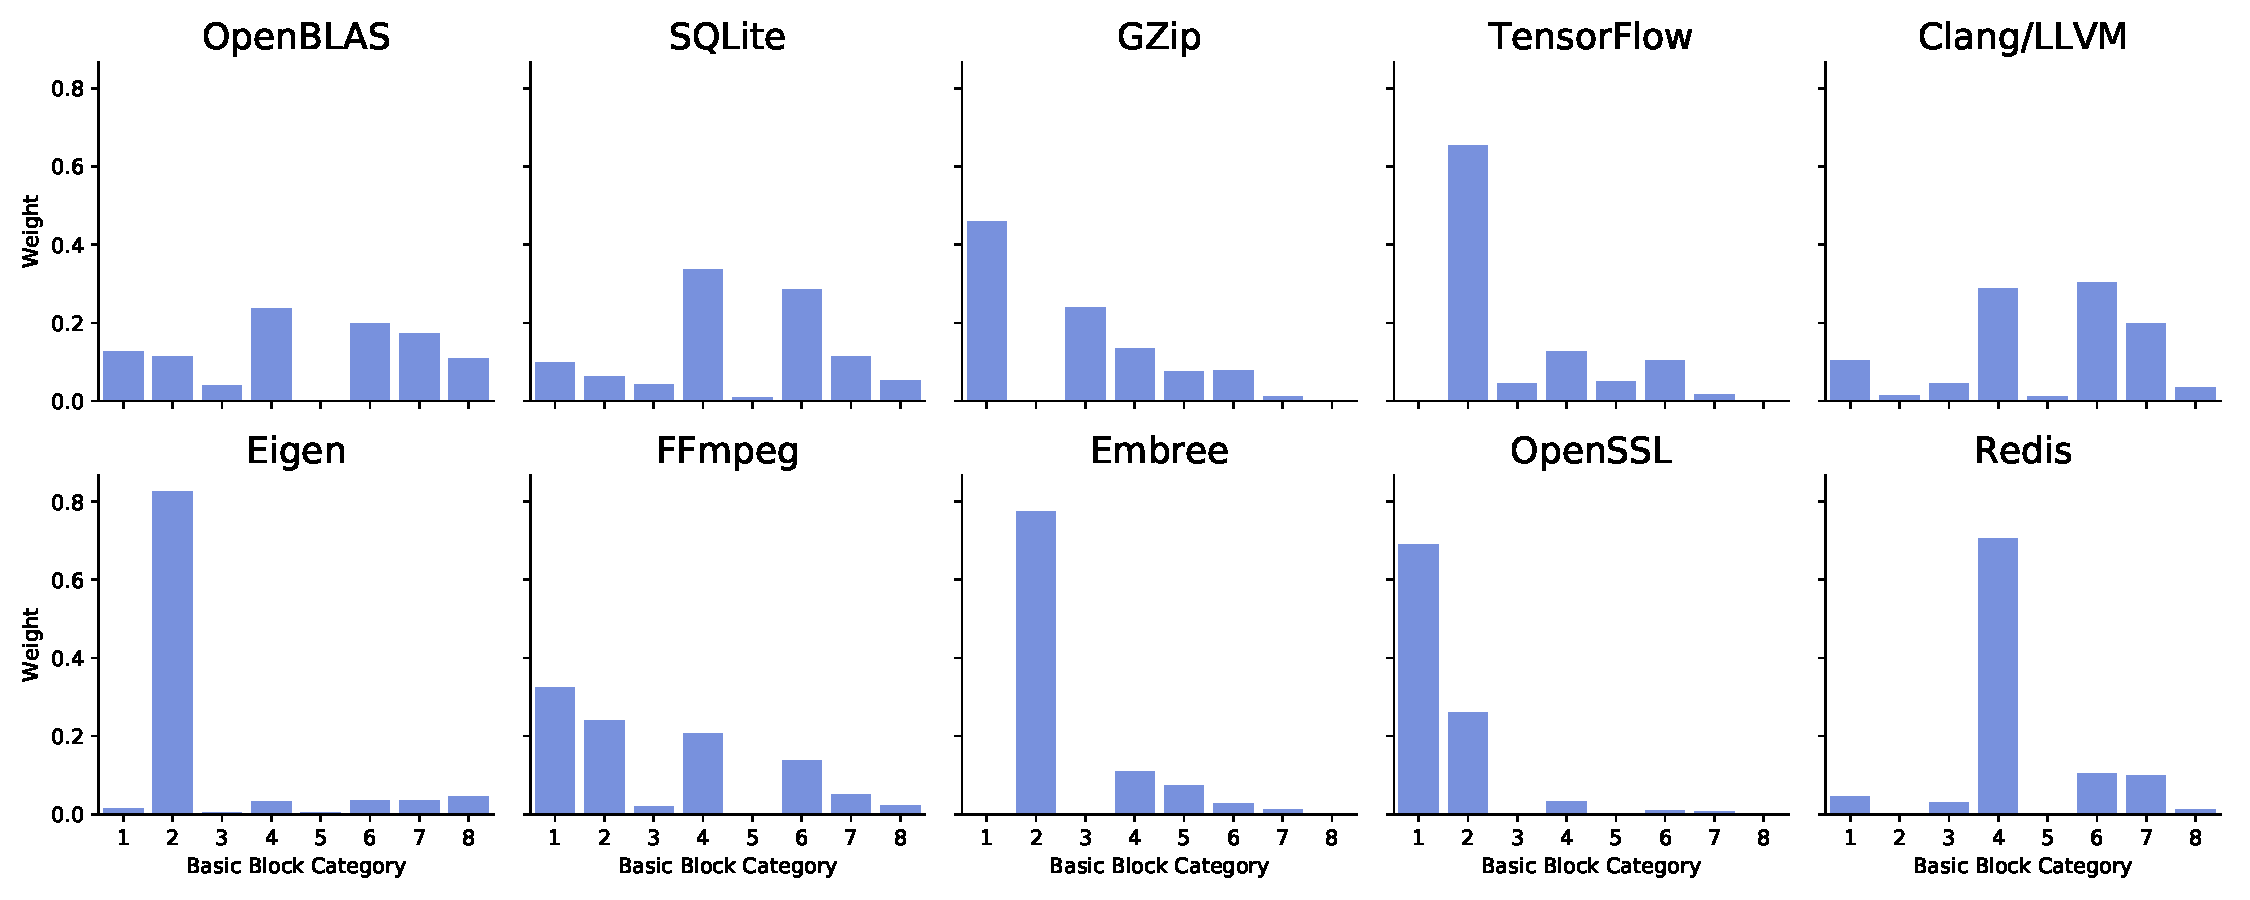
\includegraphics[width=\textwidth]{figures/apps-vs-clusters.pdf}
\caption{Breakdown of applications by basic block classes.
Y-axis represents the total weight of basic blocks
in a given class.
Category-2 contains vectorized basic blocks.
Note that the breakdown of OpenBLAS can be surprising
because the official benchmark contains
unoptimized verification code that got included into
our analysis}
\label{fig:apps_vs_clusters}
\end{figure*}